\section{Background} \label{sect:backgroundw}

In this project, we will study the performance benefits of running algorithms on the GPU in parallel. To do this we will implement three linear algebra algorithms in increasing degrees of complexity, namely: Matrix addition, matrix multiplication, and QR-decomposition.

First, we will implement these on the CPU to establish a baseline implementation. Next, we will implement them on the GPU, and hopefully see a performance increase.

This section will outline the mathematical formulas we will implement as algorithms, and the basics of CPU and GPU architecture.

\subsection{Linear Algebra}

\subsubsection{Matrix addition}

The first algorithm we want to implement is the matrix addition formula. Assume two \(m * n\) matrices \(\mathbf{A}\) and \(\mathbf{B}\). 

\[\mathbf{A} + \mathbf{B} = \mathbf{C}\]

Computing the sum of the matrices is done by adding each element \(i,j\) pairwise, where \(i\) and \(j\) are indices for the elements of the matrices.

\[a_{ij} + b_{ij} = c_{ij}\]

\begin{figure}[H]
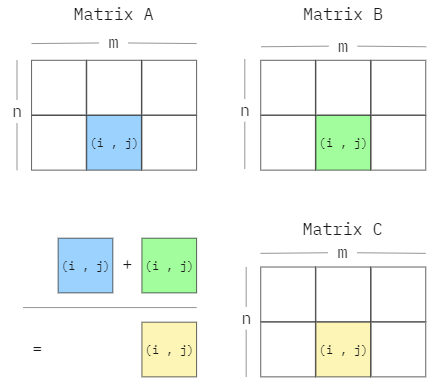
\includegraphics[scale=.65]{Documents/Report/Figures/MatrixAddition.png}
\centering
\caption{Single element addition calculation. Source: Our illustration}
\label{fig:addition_illustration}
\end{figure}

\subsubsection{Matrix multiplication}

Next we want to implement the matrix multiplication formula. Matrix multiplication \(\mathbf{A} * \mathbf{B}\) requires matrix \(\mathbf{A}\) to have dimensions \(l * m\) and matrix \(\mathbf{B}\) to have dimensions \(m * n\). This means that the column length of matrix \(\mathbf{A}\) must be equal to the row length of matrix \(\mathbf{B}\).

\[\mathbf{A} * \mathbf{B} = \mathbf{C}\]

In matrix multiplication, element \(c_{i,j}\) is calculated from the $i^{th}$ row of matrix \(\mathbf{A}\), call it \(\mathbf{A}_{i}\), and the $j^{th}$ column of matrix \(\mathbf{B}\), call it \(\mathbf{B}_{j}\). Both \(\mathbf{A}_{i}\) and \(\mathbf{B}_{j}\) have $k$ many elements. To calculate element \(c_{i,j}\), multiply each $k^{th}$ element from \(\mathbf{A}_{i}\) with \(\mathbf{B}_{j}\). Then calculate the sum of these products.

\[c_{i,j} = \sum_{k=1}^m a_{ik} b_{kj}\]

\begin{figure}[H]
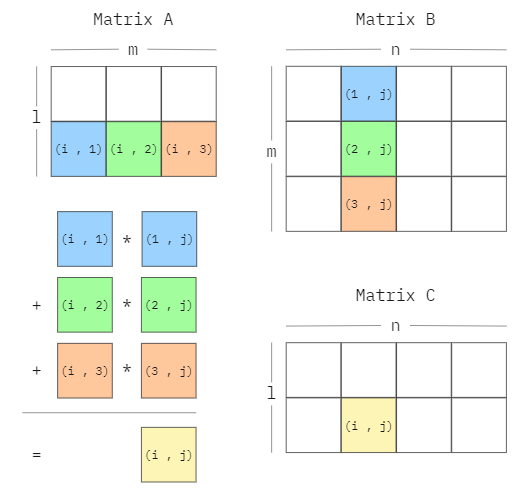
\includegraphics[scale=.65]{Documents/Report/Figures/MatrixMultiplication.png}
\centering
\caption{Single element multiplication calculation. Source: We made it}
\label{fig:multiplication_illustration}
\end{figure}

An appealing way to understand matrix multiplication is to interpret it geometrically. Assume a vector space where the unit vectors can be represented as a matrix A. To multiply this matrix with another matrix B can be interpreted such that the basis vectors are linearly transformed to new positions. For example, all vectors might be stretched by a factor of 2 and rotated clockwise by 10 degrees. 


\subsubsection{QR-decomposition}
The final algebraic algorithm we want to implement is QR-decomposition. This algorithm takes in a matrix \(\mathbf{A}\) and factorizes it into matrices \(\mathbf{Q}\) and \(\mathbf{R}\). 
\[\mathbf{A} = \mathbf{Q} * \mathbf{R}\]
Here, \(\mathbf{Q}\) is an orthogonal matrix such that 

\[\mathbf{Q^T * Q = I}\]

where \(\mathbf{Q^T}\) is the transpose of \(\mathbf{Q}\) and \(\mathbf{I}\) is the identity matrix. This property also means that \(\mathbf{Q}\) is symmetrical along the diagonal. \(\mathbf{R}\) is an upper triangular matrix, where all elements below the diagonal are 0. 

Because \(\mathbf{Q}\) is symmetrical along the diagonal and \(\mathbf{R}\) is upper triangular, the two matrices can be represented in a single matrix. In this matrix all the elements above the diagonal will be the elements of \(\mathbf{R}\) and all the elements below will be the elements of \(\mathbf{Q}\). Well almost. We don't compute the matrix Q explicitly. Instead, the householder matrices \(\mathbf{Q_i}\) for \(\mathbf{Q_0 \ldots Q_{n-1}}\) are computed for each column in our matrix \(\mathbf{A}\). Each of these will be stored in the columns below the diagonal. This leaves us with a a way to calculate \(\mathbf{Q}\) if we need it. 

\[\mathbf{Q = Q_0 * Q_1 * \ldots * Q_{n-1}}\]

Geometrically, \(\mathbf{Q}\) can be interpreted as a linear transformation that rotates and reflects the basis vectors. Likewise, \(\mathbf{R}\) can be interpreted as a linear transformation that scales and sheers the basis vectors. Therefor, by computing the QR-decomposition, we factorize a matrix into these two kinds of linear transformations. 

% What else we can include in this section on what the algorithm does

% householder vs givens
% we dont understand some of the math
% implementation from the book
% our iteration on the algorithm (TDD)
% running the loop one more time
% an iterative algorithm, the computes columns in sequence
% numerical stbility (dividing by scale)
% calculating the inner product


\newpage
\subsection{CPU and GPU Architecture}

\subsubsection{The CPU}

The chip in the computer called the \textit{Central Processing Unit} (CPU) is typically responsible for executing code. When executing code, the CPU is performing instructions on some data. That data often resides in \textit{main memory}. Main memory uses \textit{Dynamic Random Access Memory} (DRAM), which is about 10x slower than \textit{Static Random Access Memory} (SRAM). On the other hand SRAM is more expensive than DRAM in terms of production costs.\cite[p. 617-618]{computersystems} Therefor we have limited SRAM cache, while typically more DRAM available. 

A simplified overview of the CPU's architecture and its relation to main memory can be seen in figure \ref{fig:cpu_architecture}. It can be seen that the main memory is located in a physically different place than the CPU, connected by memory busses and an I/O bridge. The CPU also has a very limited on-chip storage called the \textit{cache memories}, that use SRAM.

If the CPU had to get data from main memory every time it read some data, it would slow down the computer a lot. Therefore, when the CPU reads from main memory, it also reads nearby data and writes it to its cache in anticipation that it might need it soon. When a computer program takes advantage of this, it is said to have good \textit{spatial locality}.\cite[p. 640]{computersystems}

\begin{figure}[h]
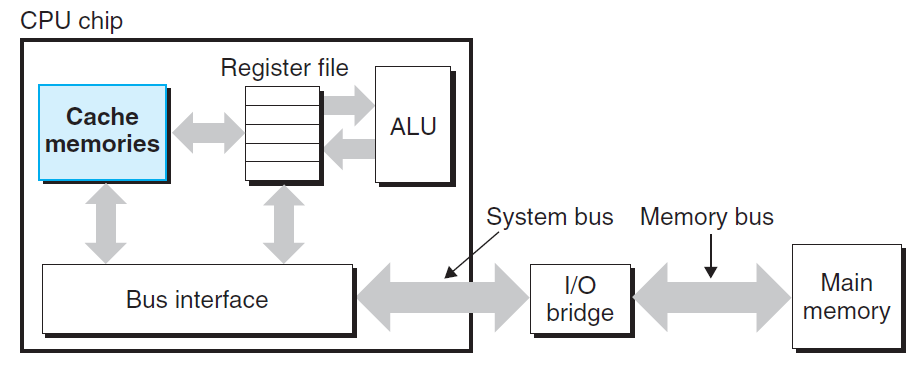
\includegraphics[width=\textwidth]{Documents/Report/Figures/CPU Architecture.png}
\caption{"Overview of CPU Architecture. Source: \cite[Figure 1.8]{computersystems}"}
\label{fig:cpu_architecture}
\end{figure}

\noindent For many years CPU cores got faster and faster. However, this development plateaued in the early 2000s. Instead, more cores were fit into the CPUs and multi-core processors were born.\cite{karlrupp:processor_trend_data}

On modern computers a CPU will contain anywhere from 2 to 90+ cores, typically in the 4-12 core range with consumer CPUs. Each core can efficiently execute a series of instructions sequentially, and each core has its own cache, as well as a shared cache between the cores.

Therefore, to run programs efficiently on a modern CPU, one should utilize all its cores by writing code which can run in parallel. This is usually done with the abstraction of \textit{threads}, which are fundamentally a sequence of instructions.\cite[p. 1022]{computersystems}\\

\subsubsection{The GPU} \label{background_gpu}

\noindent Another chip capable of executing code is called the \textit{Graphics Processing Unit} (GPU). Likewise, it has a set of cores capable of executing instructions. However, the GPU was built to process a massive amount of data in parallel. The architectural structure of the GPU is therefore different from the CPU.

The GPU is often referred to as \textit{many-core} rather than \textit{multi-core}. Instead of having a single- or double-digit amount of cores, consumer-level GPUs, usually have a three-, four- or even five-digit amount of cores, enabling many more instructions to be executed in parallel. This increase in cores comes at the cost of fewer transistors devoted to control flow and data caching as seen in figure \ref{fig:cpu_vs_gpu}.\cite[Sect. 1.1]{nvidia:cudadoc} On the GPU, memory is referred to as \textit{video random access memory} (VRAM).

\begin{figure}[ht]
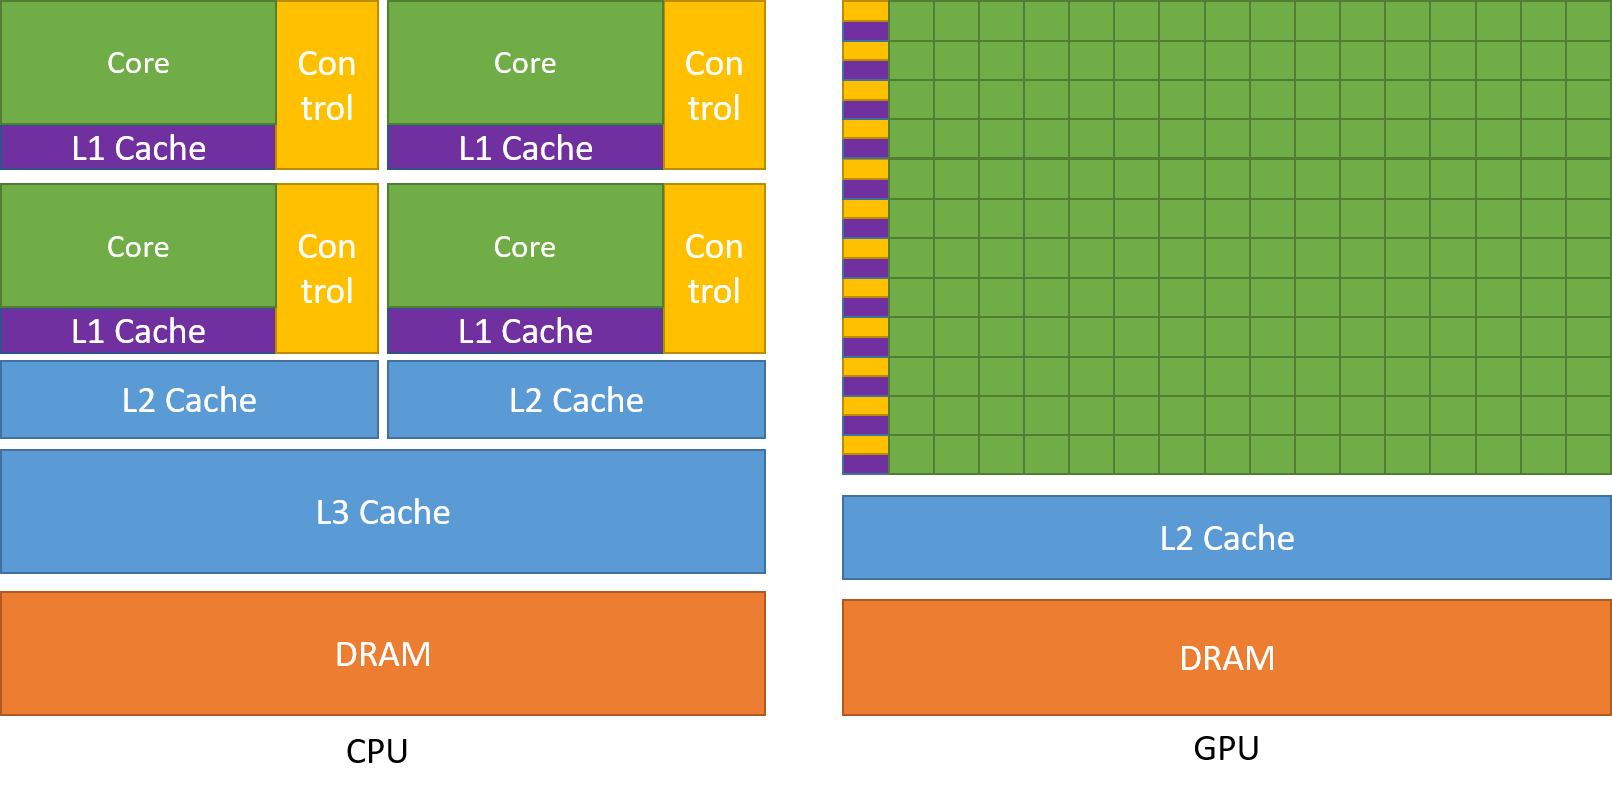
\includegraphics[width=\textwidth]{Documents/Report/Figures/CPU vs GPU .png}
\caption{"Overview of CPU Architecture and GPU Architecture. Source: \cite[Figure 1]{nvidia:cudadoc}"}
\label{fig:cpu_vs_gpu}
\end{figure}

\noindent The GPU manufacturer NVIDIA have created a parallel programming platform called CUDA. CUDA can be used in handful of languages, but for this project we use the CUDA C/C++ language extensions. These introduce some key abstractions, namely \textit{kernels, threads, thread blocks} and \textit{grids}. 

A kernel represents instructions to be executed $N$ times in parallel, where $N$ is the number of threads.[Sect. 2.1]\cite{nvidia:cudadoc} A thread executes a kernel and resides in a thread block, holding multiple threads. A thread block then resides in a grid of blocks as seen in figure \ref{fig:threads and blocks.}.

\begin{figure}[ht]
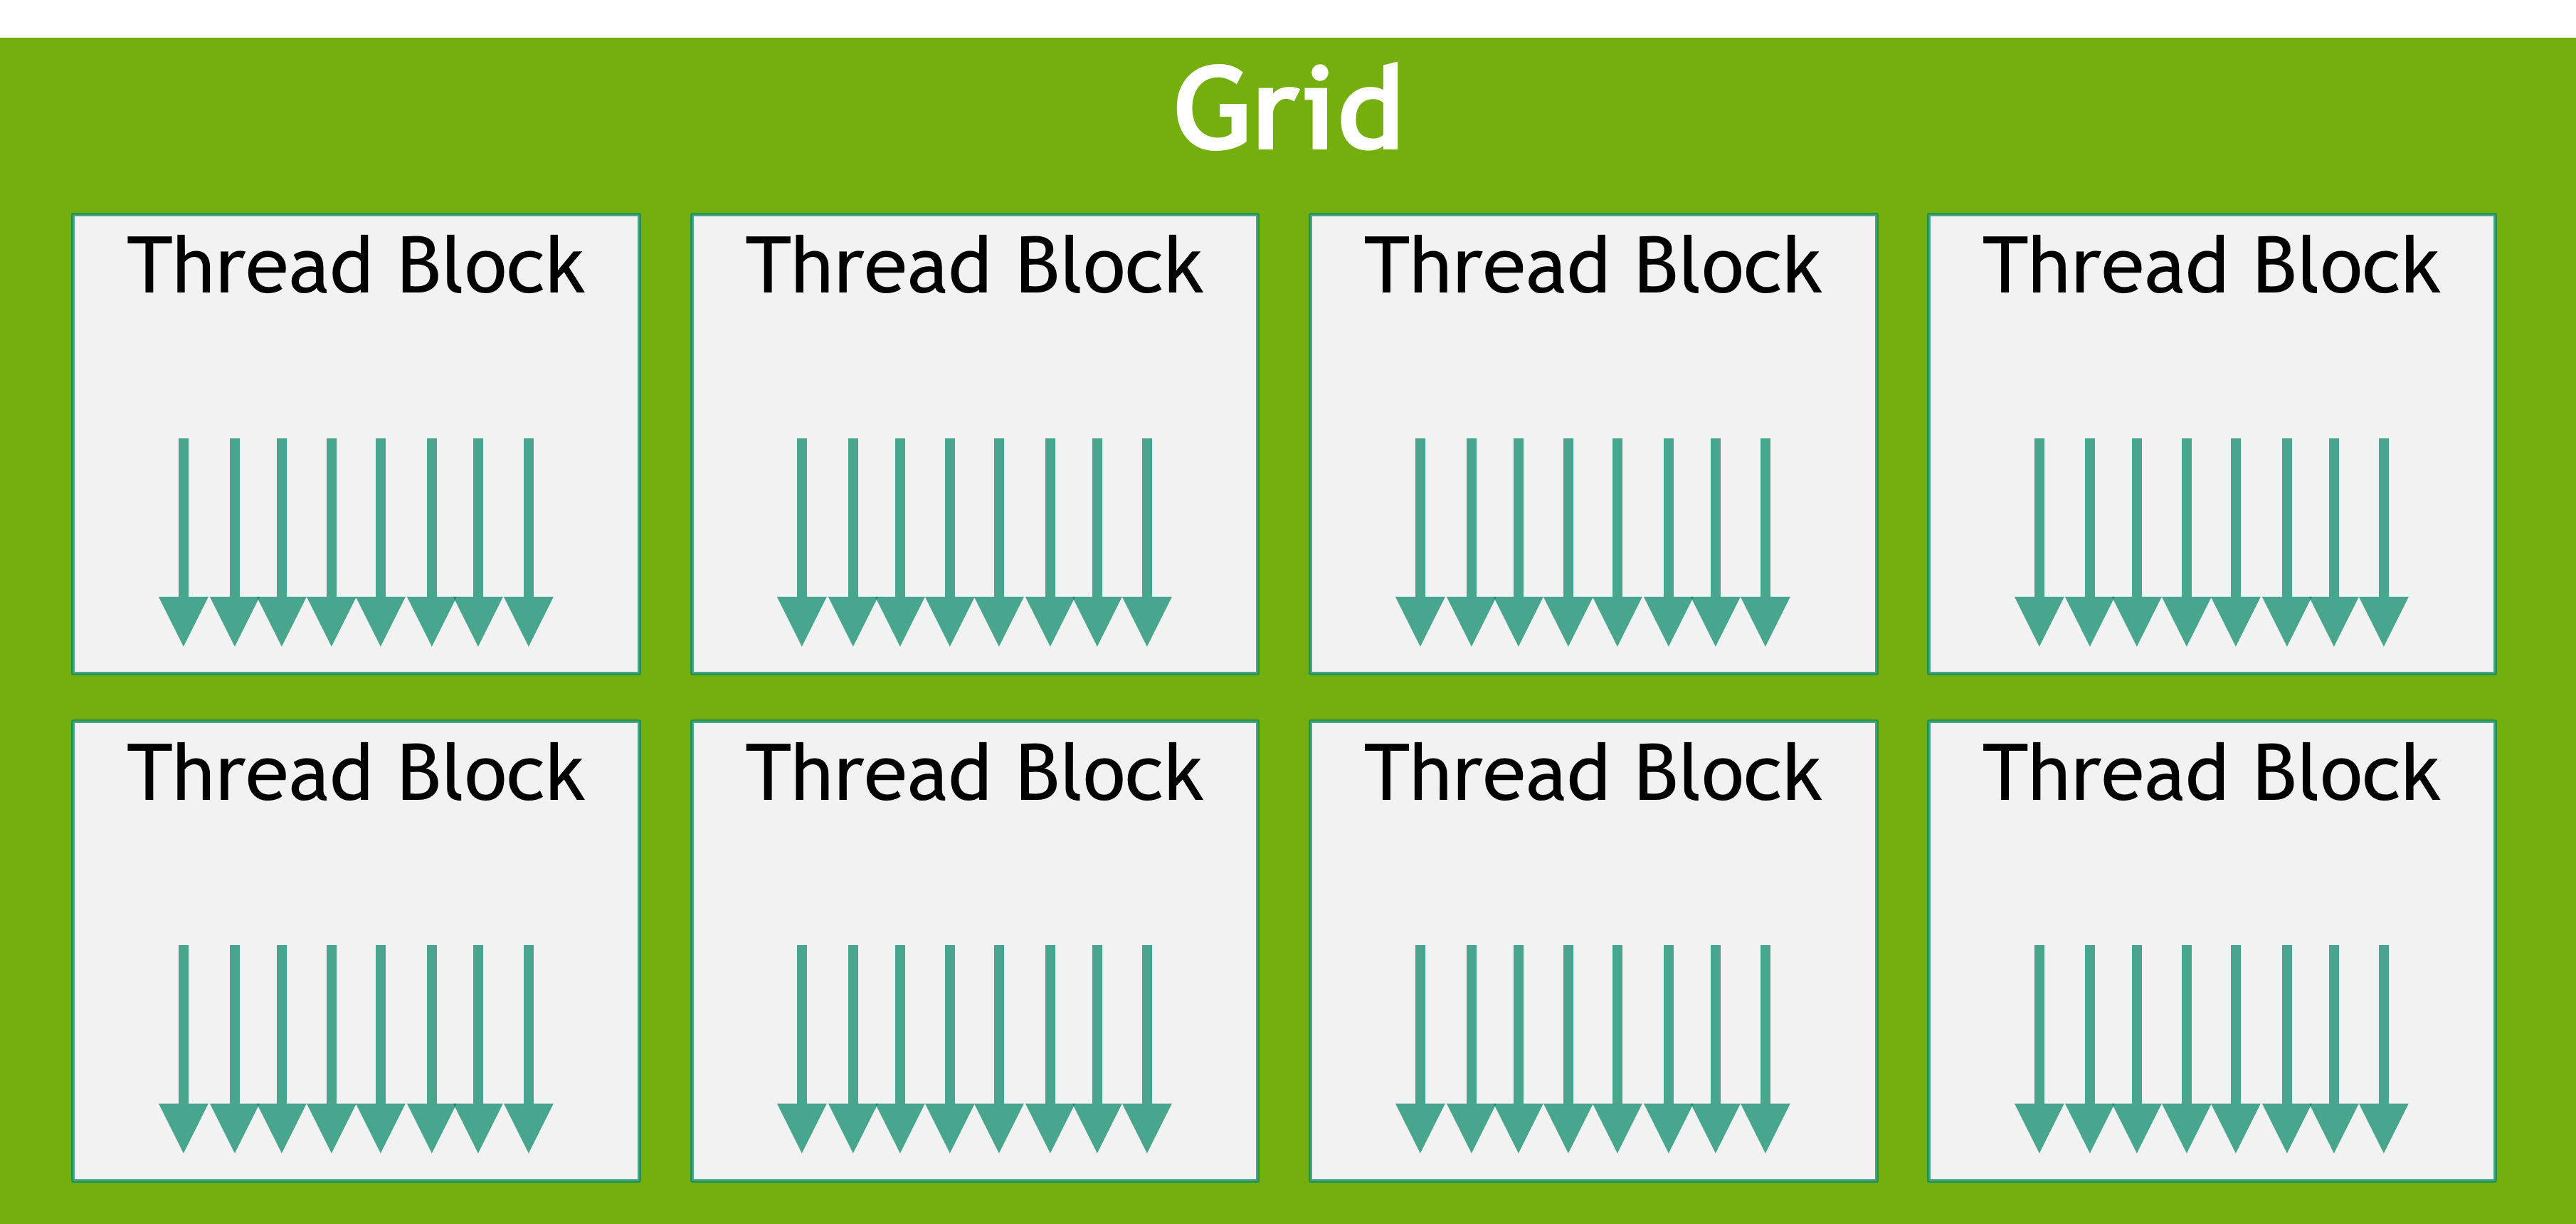
\includegraphics[width=\textwidth]{Documents/Report/Figures/Threads and blocks.png}
\caption{"Threads inside thread blocks inside the grid. Source: \cite[Figure 4]{nvidia:cudadoc}"}
\label{fig:threads and blocks.}
\end{figure}

Thread blocks and grids can be 1-, 2- or 3-dimensional. This is implemented for convenience when working with a 2-dimensional domain like matrices. A thread block can hold up to 1024 threads. The limit is there because all threads of a block is expected to be on the same \textit{streaming multiprocessor core} (SM).[Sect. 2.2]\cite{nvidia:cudadoc} The GPU is built around an array of streaming multiprocessors. Each have their own memory and control circuit, which allows threads within the same thread block to share a part of the cache, as well as synchronize with each other. 

More powerful GPUs generally have more streaming multiprocessors than less powerful GPUs. The thread block abstraction allows programmers to write efficient code for many types of GPUs, without having to worry about how many SMs they have. A GPU with more SMs will be faster, since they can execute more blocks in parallel, but both a GPU with 2 and 4 SMs will execute in parallel as fast as they are able to. This is illustrated in figure \ref{fig:automatic scalability} in appendix B.\cite[Sect. 1.3]{nvidia:cudadoc}.\\

\noindent A typical CUDA program will start with some CPU code. In this context, the CPU is called the \textit{host}. The host will likely allocate some GPU memory and copy data over to the GPU. In this context, the GPU is referred to as the \textit{device}. The host will then \textit{launch} the device kernel with special syntax: \texttt{<<<example\_kernel>>>}. When the device kernel has run, the host may then copy over some data from the device to the host and deallocate the memory on the device. So in a CUDA program, both the CPU and GPU has a role to play. 

One could say that the CPU is the manager that organizes everything, while the GPU is the hard working employee.

The typical performance bottleneck in a CUDA program is the communication between the CPU and GPU. Optimizing communication, as well as the parallelization on the GPU, is the key to optimizing performance of CUDA programs. Specifically, the transfer of data from the host memory to device memory is quite slow.\cite[Sect. 5.3.1]{nvidia:cudadoc}\\

\noindent We will implement the algorithms to run sequentially on the CPU and in parallel on the GPU. One might argue that a more fair comparison would be to write a parallel program on the CPU and then comparing the performance with the parallel program on the GPU.\footnote{One could also take advantage of SIMD operations on the CPU.}

If the purpose of the project was to judge whether an algorithm should be implemented on the CPU or GPU to yield the best performance, one would be correct. However, the purpose of this project is to implement algorithms on the GPU, and tuning that code to better performance. Writing a GPU implementation faster than a parallel implementation on the CPU is out of scope for this project.
% Talk about kernels
% 
% Talk about grids, threads, blocks, streaming multiprocessors, compute capabilities?

% Afsnit om vores hypoteser. Hvorfor vi skriver denne rapport. 
% Altså at addition ikke vil få en speedup, og hvorfor vi tror det
% at multiplication vil få en speedup, og hvorfor vi tror det
% og nogle ord om qr-decomposition 